\chapter{Tehnologii}

În cadrul acestui proiect s-au folosit următoarele tehnologii :
\begin{itemize}
\item \textbf{Unity 2019.1b} : motorul grafic folosit pentru construirea și randarea jocului.
\item \textbf{Blender} : program \textit{open source} folosit pentru modelarea 3D și contrucția obiectelor ce au fost ulterior importate în motorul grafic.
\item \textbf{Math.NET} : librărie \textit{open source} folosită pentru realizarea algoritmului de învățare automată deoarece acesta se bazează foarte mult pe lucru cu matrici.
\item \textbf{C\#} : limbajul nativ folosit de Unity pe lângă JavaScript , decizia fiind luată pur din motive de viteză.
\item \textbf{Componente din Unity} : module $built-in$ ce au ajutat la construirea aplicații de la coliziuni pănă la animații.
\end{itemize}

Din multitudinea de motoare grafice disponibile am ales \textbf{Unity} doarece e o tehnologie cu care am mai lucrat, fiind conștient de capabilitățile acestuia. Multitudinea de unelte îl fac foarte ușor de recomandat și împreună cu magazinul de \textit{assets} m-au ajutat foarte mult în procesul de construcție al acestui proiect. De asemenea \textbf{Unity} dispune de o documentație foarte bogată și bine pusă la punct , calități cheie pentru aprofundarea și folosirea acestui motor grafic.\par

Câteva exemple de sisteme ce vin la pachet cu motorul grafic ar fi, motorul de simularea a fizicii, motorul audio, sistemul de prefabricate, sistemul de iluminare și randare etc. Fără folosirea unei tehnologii ca \textbf{Unity}, acest proiect nu ar fi fost posibil într-un timp atăt de scurt , timpul de dezvoltare putând fi chiar triplat. Singurul dezavantaj imediat al acestui motor grafic este natura sa \textit{closed source}.\par

Pentru modelele 3D folosite în cadrul jocului a fost necesară folosirea unei editor și anume \textbf{Blender}. Deși mare parte din obiectele importate în joc sunt preluate de pe magazinul integrat în \textbf{Unity} , există anumite obiecte ce au fost modelate de către mine. Cu acest prilej am aprofundat anumite tehnici ce implică modelarea 3D , unul dintre cele mai importante find \textit {UV unwrapping}.\par

Am ales \textbf{Blender} datorită politcii \textit{open source} și a documentației vaste disponibile, fiind foarte ușor de lucrat în acesta, neputând aduce aplicația la un nivel dorit de finisaj fară acestă unealtă.\par

Din punct de vedere al librăriilor externe am folosit \textbf{Math.NET} , importată în \textbf{Unity} folosind \textbf{NuGet}. Necesitatea acestei librări este datorat algoritmului de invățare automată ce se bazează foarte mult pe lucrul și manipularea matricilor, de la adunarea cu un scalar până la înmulțirea/împărțirea element cu element. Detaliile legate de acest algoritm împreuna cu avantajele și dezavantajele acestuia vor fi discutate în secțiunea teoretică.\par

Datorită motorului grafic folosit și a limitărilor acestuia întregul proiect a fost construit folosind \textbf{C\#}, alternativa sa fiind \textbf{JavaScript}. Din cauza experienței cu \textbf{C\#} și a performanței ridicate am luat decizia de a folosi acest limbaj.\par

Legat de componentele folosite ce se găsesc în cadrul lui $Unity$, acestea au ajutat foarte mult la grăbirea procesului de creare a aplicației. Căteva dintre aceaste sunt \textbf{Inspector}, \textbf{WheelCollider}, \textbf{BoxCollider}, \textbf{RigidBody}, \textbf{Animator}, \textbf{Light} și multe altele.\par

\section{Structura proiectului}

Aplicația creată este împărțită în doua etape , generare și instanțiere. Din cauza unor motive de performanță fiecare zonă, deșertică, rurală și urbană are propriul său generator. De asemenea fiecare tip de platformă folosește propriul său model Markov însumând astlfel un total de șase generatori, ce se ocupă doar cu producerea unei secvențe specifice de obiecte. Pentru partea de instanțiere am fost nevoit să construiesc un sistem ce facilitează instanțierea obiectelor generate, plasândule pe platformă în sensul acelor de ceasornic.\par

Legat de structura directoarelor, \textbf{Assets} conține toate elementele necesare aplicației, de la librăria folosită pentru generarea obiectelor până la modulele de sunet și interfață iar directorul \textbf{Packages} conține cele mai importante uneltele folosite pentru realizarea și finisajul jocului importate direct de către \textbf{Unity}.\par

Aplicația fiind facută în \textbf{Unity} fișierele și directoarele au o structură arborescentă după cum urmează: \par

\dirtree{%
.1 \textbf{Assets}.
.2 \textbf{Generators}.
.2 \textbf{HMM}.
.2 \textbf{Prefabs}.
.2 \textbf{Scripts}.
.2 \textbf{Textures}.
.2 \textbf{VolumetricLights}.
.1 \textbf{Packages}.
.2 \textbf{PostProcessing}.
}
\par

\textbf{Generators} aici se află cei sașe generatori folosiți pentru construirea mediului.\par

\textbf{HMM} este directorul ce conține scripturile necesare pentru construirea modelului Markov și a antrenării lui.\par

\textbf{Prefabs} este directorul cu toate prefabricatele din joc, incluzând modelele pentru platforme, obiecte, jucător cât și inamici.

\textbf{Scripts} aici sunt stocate toate fișierele sursă ce modelează comportamentul jucatorului, al meniurilor și a sistemelui de generare/instanțiere, sumându-se în total la optsprezece fișiere.\par

\textbf{Textures} directorul ce conține toate fișierele de tip \textit{Albedomap} , \textit{Heightmap} și \textit{Occlusionmap} folosite în cadrul materialelor ce au fost ulterior importate pe obiecte.\par

\textbf{VolumetricLights} directorul ce conține fișierele preluate de pe \textit{Github} pentru lumină volumetrică.\par

\textbf{PostProcessing} modulul folosit de \textit{Unity} pentru a putea integra efecte precum corectare de culoare, \textit{bloom}, \textit{motion blur} și multe altele.\par


\section{Componente}
Aplicația prezentă este împărțită pe diferite module ce controlează sunetul, generarea, \textit{UI-ul} , instanțierea și multe altele. În \textbf{Unity} acest lucru se realizeză în mare parte prin fișiere sursă atașate de obiectele din scena curentă. \par

Am optat să construiesc jocul în jurul unei singure scene, ceea ce necesită un numar mai mare de operatori și fișiere sursă. O consecință directă a folosirii unei singure scene este integrarea meniului principal în același mediu ca și jocul în sine. De aici derivă necesitatea de două scripturi ce controlează tranziția de la meniu la joc intitulate sugestiv \textit{MenuController} și \textit{GameController}.\par


\begin{figure}[H]
\centering
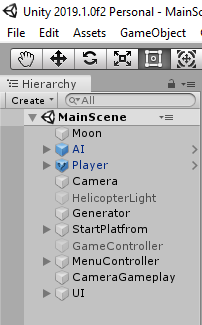
\includegraphics[width=0.5\linewidth]{Structure.png} \par
\caption{Structura arborescentă a obiectelor din scenă}
\end{figure}

De asemenea există un obiect \textit{Generator} ce conține toți generatori necesari pentru construirea scenei. Unul pentru fiecare tip de zonă de interes și tip de platformă. Legătura între cei sașe generatori este facută de cele două scripturi atașate de obiectul \textit{Camera} denumite \textit{PlatformBuilder} și \textit{PlatformController}. Primul se ocupă cu instanțiera și plasarea obiectelor pe platformă în funcție de parametri de instanțiere setați de un script atașat de un \textit{Spawn Point}. Cel de-al doilea se ocupă cu randomizarea și controlarea numărului de platforme pentru fiecare zonă de interes.\par
\par

\subsection{MenuController}

Acest obiect se ocupă de toate aspectele ce țin de meniul principal. Deoarece există o singură scenă scriptul este destul de complex, rolul său fiind activarea tuturor componentelor ce țin de jocul principal, sunet, inamici, jucător, cameră, efecte și multe altele.\par

În continuare se vor prezenta cele mai importante secvențe de cod ce se găsesc în fișierul \textbf{MenuController}.\par

\begin{lstlisting}[caption=Funcțiile din MenuController]
public void OnGameExit(){
        Application.Quit();
}
public static void OnGameReset(){
        retry = true;
}
public void OnCredits(){
        this.creditsStart = true;
        this.credits.SetActive(true);
}
public void OnGameStart(){
        gameStart = true;
        gameController.SetActive(true);
        player.constraints = RigidbodyConstraints.None;
        AI.constraints = RigidbodyConstraints.None;
        player.velocity = Vector3.forward * 3;
        AI.velocity = Vector3.forward;
        bars.SetActive(true);
}
\end{lstlisting}

Cele patru funcții controlează tranzițiile aplicației în funcție de interacțiunea jucatorului cu meniul principal. De remarcat în funcția \textit{OnGameStart} linia ce activează \textit{GameController} odată ce se pornește jocul și anume \textit{gameController.SetActive(true)}.\par

\subsection{GameController}

Obiectul ce se ocupă de funcționalitatea principală din joc. În mare parte meniul de pauză și meniul de final al jocului sunt controlate de acest script.\par

Legat de parte de cod, fișierul sursă atașat de obiect arată astfel:\par

\begin{lstlisting}[caption=Funcțiile din GameController,
  label=a_label]
public void SetPausedState(){
        gamePaused = gamePaused == true ? false : true;
}
public void SetGameOverState(){
        player.GetComponent<CarController>().enabled = false;
        cameraScript.enabled = false;
        enemyScript.enabled = false;
        gameOver = true;
        gameOverScreen.SetActive(true);
}
public void TogglePause(){
        ToggleSound();
        ToggleRender();
        TogglePauseMenu();
        SetPausedState();
}
\end{lstlisting}

Meniul din joc odată activat oprește actualizarea grafică a jocului, lucru ce complică apelu de funcții dependente de timp.\par

\subsection{PlatformBuilder}

Scriptul ce realizează construirea în timp real a platformelor și le instanțiază. Datorită volumului mare de cod mai jos este prezentată doar funcția ce adaugă obiectele pe platformă. Înainte de instanțiere funcția are grija să preia datele de \textit{spawn}, conținute de scriptul atașat \textit{SpawnSettings} pentru fiecare loc valid de instanțiere.\par

\begin{lstlisting}[caption=Funcțiile din PlatformBuilder,
  label=a_label]
public GameObject BuildPlatform(GameObject state){
        GameObject nextPlatform = Instantiate(state, new Vector3(currentPlatform.transform.position.x + xOffset, -15, currentPlatform.transform.position.z + zOffset), Quaternion.Euler(0, 0, 0));
        HMM propGenerator = ChoosePropGenerator(nextPlatform.name);
        Transform spawnPoints = nextPlatform.transform.Find("SpawnPoints");
        foreach (Transform spawn in spawnPoints){
            SpawnSettings spawnSettings = spawn.GetComponent<SpawnSettings>();
            if (spawnSettings.isStackable == false && spawnSettings.maxObjectStack > 1)
                throw new System.Exception("Spawn is not stackable!");
            for (int i = 0; i < spawnSettings.maxObjectStack; ++i){
                InstantiateProp(propGenerator, spawn, spawnSettings, i);
            }
        }
        nextPlatform.transform.rotation = Quaternion.Euler(0, rotation, 0);
        return nextPlatform;
}
\end{lstlisting}

Scriptul \textit{SpawnSettings} conține doi parametri \textit{isStackable} și \textit{maxObjectStack} folosite pentru a specifica dacă locul de \textit{spawn} poate să conțină mai multe obiecte și în ce cantitate.\par

\subsection{PlatformController}

Din cauza necesității de a controla durata unei anumite zone evitănd astfel inconsistența, \textit{PlatformController} alege un număr de platforme pentru fiecare secțiune ținând cont de o limită superioară și inferioară.\par

\begin{lstlisting}[caption=Funcțiile din PlatformController,
  label=a_label,
  mathescape=false]
public GameObject GetNextPlatform(){
        GameObject output;
        currentEmissionCount++;
        if (currentEmissionCount > maxEmissionCount){
            output = transitionPlatforms[currentGeneratorIndex];
            currentEmissionCount = 0;
            currentGeneratorIndex = (currentGeneratorIndex + 1) % generators.Length;
            maxEmissionCount = Random.Range(lowerBound, upperBound);
        }
        else{
            output = generators[currentGeneratorIndex].NextEmission();
        }
        return output;
}
\end{lstlisting}
